\chapter{Implementación}

Neste capítulo se comentarán os aspectos máis relevantes da implementación da nosa plataforma.


\section{Servidor}
Nesta sección vanse tratar todos os detalles de implementación propios do servidor, dende o acceso á base de datos ata a construción dos servizos web. En todo o servidor utilizouse a ferramenta de Spring para configurar a transaccionalidade, a inxección de dependencias, ou a creación dos servizos web.
A autenticación con Google terá a súa propia sección ao final do capítulo.


AWS.

\subsection{Acceso á base de datos}
Para o acceso á base de datos utilizouse directamente JDBC sen facer uso de ningunha ferramenta de mapeo obxecto-relacional como pode ser Hibernate. Escolleuse esta opción por ser un sistema sen moita complexidade á hora de gardar ou eliminar rexistros en base de datos e cun número de táboas non moi alto. En sistemas pequenos non se aproveitan os beneficios que poden ter estas ferramentas e desta maneira afórrase a súa configuración.

Creouse unha implementación para cada un dos DAOs amosados na sección de deseño. Dentro deles fanse todas as accións permitidas sobre as táboas que representa cada VO.

Exemplo de inxección de consulta

Exemplo de execución de consulta








\subsection{Transaccionalidade}
A xestión transaccionalidade impleméntase na capa Manager utilizando o framework Spring, grazas á súa librería spring-tx. A súa configuración e utilización é moi sinxela, tal e como se pode observar nos exemplos. No primeiro amósase a configuración que require nos ficheiros XML de Spring. Para indicar a transaccionalidade, utilizaremos etiquetas que permitan identificar o tipo de transacción que queremos que se aplique en cada método público do manager. Non todos os métodos provocan escrituras en base de datos, polo que non será necesario indicar o tipo de transaccionalidade que provoca desfacer cambios en todos eles. O resto marcaranse como de só lectura para non sobrecargar innecesariamente o sistema.

Na figura~\ref{fig:transaccionConfiguracion} pódese observar a configuración da transaccionalidade nos ficheiros XML.

\begin{figure}[tbh] 
	\begin{center}
		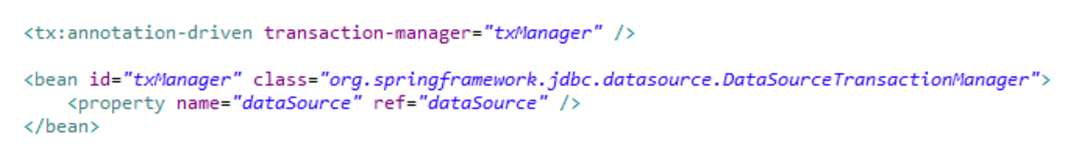
\includegraphics[width=1\textwidth]{figures/codigo/transaccionConfiguracion}
		\caption{Configuración da transaccionalidade no ficheiro XML.}
		\label{fig:transaccionConfiguracion}
	\end{center}
\end{figure}


Na figura~\ref{fig:metodoTransaccional} pódese observar a configuración da transaccionalidade sobre un método no que se modifican datos.

\begin{figure}[tbh] 
	\begin{center}
		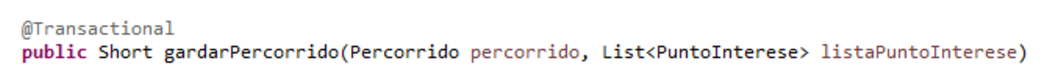
\includegraphics[width=1\textwidth]{figures/codigo/metodoTransaccional}
		\caption{Configuración da transaccionalidade dun método onde se modifican datos.}
		\label{fig:metodoTransaccional}
	\end{center}
\end{figure}

Na figura~\ref{fig:metodoNonTransaccional} pódese observar a configuración da transaccionalidade sobre un método de só lectura.

\begin{figure}[tbh] 
	\begin{center}
		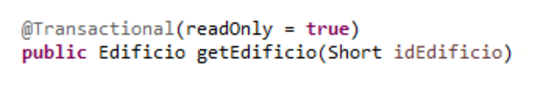
\includegraphics[width=0.5\textwidth]{figures/codigo/metodoNonTransaccional}
		\caption{Configuración da transaccionalidade dun método de só lectura.}
		\label{fig:metodoNonTransaccional}
	\end{center}
\end{figure}


\subsection{Construción dos servizos web}
Para a construción dos servizos web creáronse dous controladores distintos, tal e como se comentou na sección de deseño: un para as imaxes e o outro para o resto de información. Esta capa comúnicase coa capa dos manager, detallada na subsección anterior \todo{ligazon?}. Para a súa implementación usouse unha librería específica de Spring para a construción de servizos web: Spring MVC.


Exemplo de construción dos servizos web: Spring MVC















\section{Aplicación Android}
Nesta sección trataranse os aspectos máis importantes da implementación na aplicación Android.
\subsection{Solicitude de permisos}
Como se solicitan permisos na aplicación
Non fan falla na instalación. Solicítanse na execución. Sen o permiso de localización non funcionaría a aplicación.

\subsection{Acceso a Situm}
Para o acceso aos servizos de Situm optouse por illar as conexións en clases distintas para non mesturar lóxica. Estes accesos realizáronse mediante o uso da SDK de Situm na súa versión \todo{mirar versión}.

Exemplo de acceso a Situm

\subsection{Acceso ao servidor}
Ao igual que se explicou no punto anterior, a conexión co servidor propio realizouse mediante conexións illadas en distintas clases. 
Exemplo de acceso ao servizo web




Exemplo de chamada a actividade e devolución do fluxo

Para publicar a aplicación na Play Store
https://developer.android.com/studio/publish/app-signing




\section{Autenticación}
Neste punto verase o proceso de autenticación en máis profundidade, revisando as diferentes chamadas necesarias tanto dende a aplicacion Android coma dende o servidor contra os servizos de Google para verificar a identidade do usuario.




https://developers.google.com/identity/sign-in/android/start-integrating


https://developers.google.com/android/guides/client-auth


Incluír o google-services.json dentro da aplicación Android para permitir a conexión